\section{Praktyczne problemy}
W tej sekcji zostaną przedstawione przypadki zastosowania teoretycznej wiedzy wraz z praktycznymi przykładami.



\subsection{Sortowanie wyników}
Załóżmy, że chcemy uzyskać wyniki zapytania posortowane według pewnej kolejności. Jest to oczywiście pewien dodatkowy nakład, który serwer MySQL musi wykonać podczas wykonania zapytania.

Podstawą optymalizacji sortowania jest używanie indeksów typu B-Tree, ponieważ indeks jest posortowany względem jego kolumn. Aby przedstawić działanie indeksu na rzeczywistich przykładach, użyto bazy \text{StackOverflow}. Z bazy usunięto wszystkie indeksy oraz klucze główne założone na wykorzystywanych w przykładach tabelach, aby nie wpływały one na prezentowane przykłady.


Najlepszym z możliwych scenariuszy wykorzystania indeksu do sortowania danych jest sytuacja, kiedy kolumny użyte do sortowania odpowiadają indeksowi, a kolumny, które chcemy zwrócić jako wynik zapytania, są podzbiorem kolumn indeksu.
Weźmy tabelę Users, na którą założono indeks typu BTREE jak poniżej.

\begin{spverbatim}
	CREATE INDEX Rank_idx ON Users(Reputation, UpVotes);
\end{spverbatim}
Następnie wykonano następujące zapytanie.
\begin{spverbatim}
	EXPLAIN SELECT Reputation,UpVotes FROM Users ORDER BY Reputation, UpVotes;
\end{spverbatim}
Dla tego zapytania polecenie EXPLAIN zwróci w kolumnie EXTRA informację: "Using index", co oznacza, że do sortowania wartości użyto indeksu znajdującego się w kolumnie key, czyli indeksu, który został stworzony przed wykonaniem zapytania.

\begin{figure}[H]
	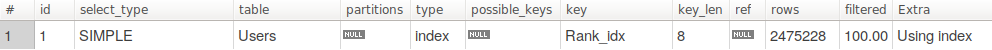
\includegraphics[scale =0.4]{explain15.png} 
\end{figure}
Jeżeli w wyniki chcemy otrzymać jedynie kolumnę \textit{Reputation}, to MySQL wciąż będzie wykorzystywał indeks do sortowania wyników, ponieważ spełnia to warunek zawierania się kolumn rezulatu zapytania w zbiorze kolumn indeksu. W kolejnym kroku sprawdzono, co się stanie, jeżeli do klauzuli WHERE zostanie dodana kolejna kolumna.
\begin{spverbatim}
	EXPLAIN SELECT Id, Reputation, UpVotes FROM Users ORDER BY Reputation, UpVotes;
\end{spverbatim}
\begin{figure}[H]
	
\includegraphics[scale =0.4]{explain16.png} 
\end{figure}
Tym razem MySQL nie wykorzystał indeksu, ale pobrał wszystkie dane i posortował, wykorzystując jeden z dostępnych w MySQL algorytmów sortowania. Co ciekawe, nie zawsze musi się tak stać. MySQL na etapie analizy wykonania sprawdza, czy wydajniejsze będzie dla niego sortowanie wyników na podstawie pobranych danych, czy może, jeżeli sortujemy dane względem jednego z indeksów na tabeli, pobrać ten indeks i wykorzystać do wydajniejszego sortowania.

Następnie dodano klucz główny dla tabeli Users i sprawdono, co się stanie, jeżeli zostanie umieszczony jako jedna z kolumn wyniku zapytania.
\begin{spverbatim}
	ALTER TABLE Users ADD PRIMARY KEY (Id);
	EXPLAIN SELECT Id, Reputation, UpVotes FROM Users ORDER BY Reputation, UpVotes;
\end{spverbatim}

\begin{figure}[H]
	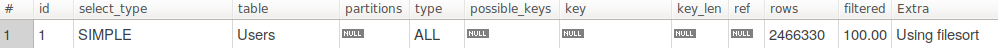
\includegraphics[scale =0.4]{explain17.png} 
\end{figure}
Wynik polecenia EXPLAIN jest interesujący. Przypomnijmy sobie zatem, w jaki sposób MySQL przechowuje dane w indeksie, jeżeli tabela posiada klucz podstawowy. Wtedy wiersze w liściach indeksu są identyfikowane za pomocą wartości kluczy głównych. W rozważanym przypadku wiersze w indeksie są identyfikowane na podstawie kolumny \textit{id}, co oznacza, że indeks zawiera wszystkie kolumny użyte w zapytaniu.
Dzięki temu aby uzyskać wynik serwer nie musi odwoływać się do dysku, aby pobrać dane, ponieważ wszystkie dane użyte w zapytniu znajdują się w indeksie. Jest to przykład wykorzystania indeksu pokrywającego.

Kolejnym często używanym zapytaniem jest pobranie wszystkich kolumn z tabeli, ale sortowanie ich według określonych kolumn. Weźmy następujące zapytanie:
\begin{spverbatim}
	EXPLAIN SELECT u.* FROM Users u ORDER BY u.UpVotes, u.Reputation;
\end{spverbatim}
Tym razem MySQL znów najprawdopodobniej nie użyje indeksu do posortowania danych, ponieważ kolejność kolumn użytych do sortowania danych nie jest identyczny jak w indeksie.

W kolejnym przykładzie przeanalizowano następujące zapytanie.
\begin{spverbatim}
	EXPLAIN SELECT * FROM Users WHERE Reputation = 1 ORDER BY UpVotes;
\end{spverbatim}
\begin{figure}[H]
	
\includegraphics[scale =0.4]{explain18.png} 
\end{figure}
Tym razem MySQL znów wykorzystał indeks, do posortowania wyników, ponieważ kolumny w indeksie są posortowane względem kolumn Reputation, a w przypadku, kiedy wartość Reputation jest równa, względem kolumny UpVote, co odpowiada wartości ORDER BY.
Następnie sprawdzono co się stanie po delikatnej modyfikacji zapytania do postaci:
\begin{spverbatim}
	EXPLAIN SELECT * FROM Users WHERE Reputation > 1000 ORDER BY UpVotes;
\end{spverbatim}

W tym przypadku nie ma jednoznacznej odpowiedzi na pytanie, w jaki sposób MySQL posortuje dane. Optymalizator MySQL musi podjąć decyzję, czy warunki w klauzuli WHERE są wystarczająco selektywne, czy może pobranie indeksu i na jego podstawie przeprowadzenie sortowania będzie efektywniejsze.

\subsection{Przechowywanie wartości NULL czy pustej wartości}
Częstym zagadnieniem dotyczącym przechowywania danych w tabelach MySQL jest pytanie, w jaki sposób reprezentować brak wartości. Załóżmy, że mamy tabelę studentów, która posiada wiersz z numerem domowym studenta. Zdecydowana większość studentów nie posiada numeru domowego. W jaki zatem sposób ustawić wartość w bazie danych? Brak numeru zapisać jako wartość NULL czy może pusty ciąg znaków? Na początku rozważono kwestię wykorzystania przestrzeni na dysku. Przygotowano cztery następujące tabele:

\begin{spverbatim}
	CREATE TABLE test_null_varchar_values(
	k1 varchar(32) not null, k2 varchar(32) not null,
	k3 varchar(32) not null, k4 varchar(32) not null,
	k5 varchar(32) not null, k6 varchar(32) not null,
	k7 varchar(32) not null, k8 varchar(32) not null);
	
	CREATE TABLE test_not_null_varchar_values(
	k1 varchar(32) not null, k2 varchar(32) not null,
	k3 varchar(32) not null, k4 varchar(32) not null,
	k5 varchar(32) not null, k6 varchar(32) not null,
	k7 varchar(32) not null, k8 varchar(32) not null);
	
	CREATE TABLE test_not_null_int_values(
	k1 int not null, k2 int not null,
	k3 int not null, k4 int not null,
	k5 int not null, k6 int not null,
	k7 int not null, k8 int not null);
	
	CREATE TABLE test__null_int_values(
	k1 int,	k2 int,	k3 int, k4 int,
	k5 int,	k6 int,	k7 int,	k8 int);
	
\end{spverbatim}

Następnie tebele zostały wypełnione piętnastoma tysiącami wierszy. W przypadku tabeli, które dopuszczają wartość NULL wypełniono je takimi właśnie wartościami. Dla tabel z kolumnami oznaczonymi jako NOT NULL wypełniono odpowiednio pustym tekstem ('') lub wartością 0.
Następnie na każdej z tabel wykonano polecenie ANALYZE TABLE, w celu aktualizacji statystyk i wykonano polecenie SHOW TABLE STATUS, którego wyniki umieszczono poniżej na rysunku ~\ref{fig:null_vs_empty_value_analyze_table}.

\begin{figure}
	\caption{Wyniki polecenia SHOW TABLE STATUS dla tabeli z ośmioma kolumnami}
	\centering
	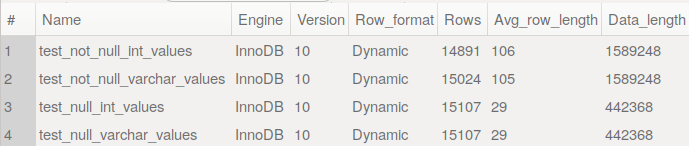
\includegraphics[scale = 0.43]{null_vs_empty_value_analyze_table.png}
	\label{fig:null_vs_empty_value_analyze_table}
\end{figure}

Wykorzystanie NULL zredukować rozmiar tabel o ok. 70 \%. W kolejnym kroku przeanalizowano sytuację, kiedy w tabeli przechowywana jest tylko jedna kolumnę z możliwymi wartościami NULL. Zmodyfikowano skrypty tworzące tabele tak, żeby każda tabela posiadała tylko jedną kolumnę. W analogiczny sposób wypełniono bazę piętnastoma tysiącami wierszy i dla każdej z tabel wykonano polecenie ANALYZE TABLE. Na rysunku ~\ref{fig:null_vs_empty_value_analyze_table_for_one_column} przedstawiono wyniki polecenia SHOW TABLE STATUS dla tabeli.

\begin{figure}
	\caption{Wyniki polecenia ANALYZE TABLE dla tabeli z jedną kolumną}
	\centering
	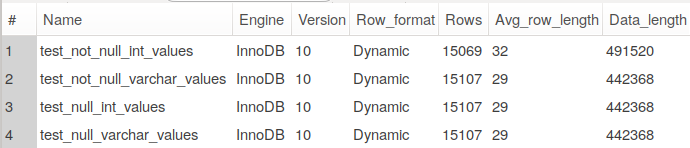
\includegraphics[scale = 0.43]{null_vs_empty_value_analyze_table_for_one_column.png}
	\label{fig:null_vs_empty_value_analyze_table_for_one_column}
\end{figure}

Jednakowy rozmiar wierszy zawierających osiem wartości NULL oraz wierszy z jedną wartością NULL wynika ze sposobu w jaki MySQL przechowuje informację o kolumnach z wartościami NULL. Dla każdego wiersza, który zawiera kolumny z wartości przechowywany, jest dodatkowy bajt z informacją o kolumnach z wartością NULL. MySQL na każdym bajcie przechowuje informacje dla maksymalnie 8 kolumn (jeden bit dla każdej z kolumn). Gdyby w wierszu zawierającym osiem kolumn, dodana została jeszcze jedna kolumna z dopuszczalną wartością NULL, wtedy MySQL zarezerwowałby dodatkowy bajt dla tego wiersza.


\subsection{Indeks na wielu kolumnach czy wiele indeksów na jednej}
Przed wersją 5.0 MySQL pozwalał na użycie tylko jednego indeksu dla tabeli, nawet jeżeli potencjalnie użytecznych było więcej. W takim przypadku, aby wyszukiwanie na większej liczbie kolumn korzystało z indeksów, należało utworzyć indeks składający się z wilu kolumn. W wersji 5.0 wprowadzony został algorytm łączenia indeksów (\textit{index merge}). Idea łączenia indeksów umożliwia łączenie różnych indeksów na kolumnach użytych w klauzuli WHERE. Jako przykład posłużono się tabelą \textit{Users} z bazy \textit{StackOverflow}. Na początku założono dwa osobne indeksy na kolumny \textit{reputation} oraz \textit{views} i wykonano analizę zapytania wyszukującego dane z wykorzystaniem obu kolumn.
\begin{spverbatim}
	CREATE INDEX reputation_idx ON Users(reputation);
	CREATE INDEX views_idx ON Users(views);
	EXPLAIN SELECT count(*) FROM Users where reputation = 1 and views = 1;
\end{spverbatim}
\begin{figure}
	\caption{Wyniki polecenia ANALYZE TABLE dla dwóch indeksów}
	\centering
	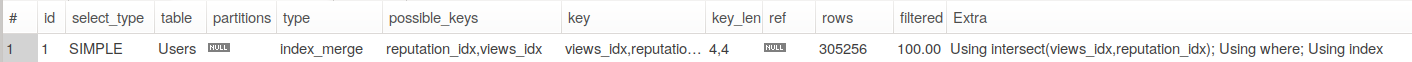
\includegraphics[scale = 0.32]{explain_merge_index.png}
	\label{fig:explain_merge_index}
\end{figure}

Następnie zastąpiono pojedyncze indeksy jednym wielokolumnowym i wykonano analogiczną analizę.
\begin{spverbatim}
	EXPLAIN SELECT COUNT(*) FROM Users WHERE reputation = 1 AND views = 1;
\end{spverbatim}

\begin{figure}
	\caption{Wyniki polecenia ANALYZE TABLE dla pojedyńczego indeksu}
	\centering
	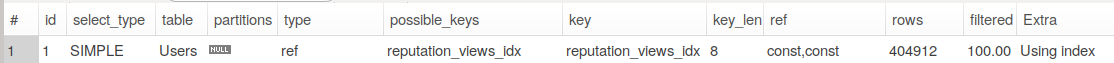
\includegraphics[scale = 0.32]{explain_without_merge_index.png}
	\label{fig:explain_without_merge_index}
\end{figure}

Na rysunkach ~\ref{fig:explain_merge_index} oraz ~\ref{fig:explain_without_merge_index} zaprezentowano wynyniki polcenia EXPLAIN dla obu przypadków. W obu odfiltrowane zostało 100 \% wierszy. W następnej kolejności zmierzono średni czas wykonania obu zapytań. W przypadku pojdeńczego indeksu zapytanie wymagało śrendio 0.05 sekundy, natomiast przy łaczeniu tabel ok. 0.5 sekundy. Na koniec usunięto indeks dla kolumny \textit{Views}, żeby optymalizator wykorzystał tylko indeks \textit{reputation\textunderscore idx}.
\begin{spverbatim}
	CREATE INDEX reputation_idx ON Users(reputation);
	EXPLAIN SELECT COUNT(*) FROM Users WHERE reputation = 1 AND views = 1;
\end{spverbatim}
\begin{figure}[h!]
	\centering
	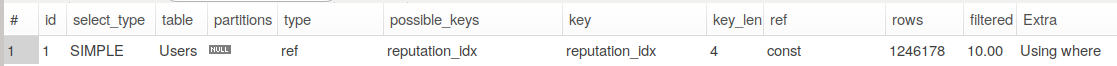
\includegraphics[scale = 0.32]{explain_with_reputation_idx.png}
	\caption{Wyniki polecenia ANALYZE TABLE dla indeksu \textit{reputation\textunderscore idx}}
	\label{fig:explain_with_reputation_idx}
\end{figure}

Tym razem tylko 10 \% wierszy zostało odfiltrowane, a średni czas wykonania zapytania zbliżył się do 8 sekund. Analizując wyniki powyższego eksperymentu można stwierdzić, że mechanizm łaczenia tabel nie będzie równie wydajny co pojedyńczy indeks na wielu kolumnach, ale może być dobrą alternatywą do pełnego przeszukania lub wykorzystania jedynie jednego indeksu.
\subsection{Sztuczny czy naturalny klucz główny}
TODO

\subsection{Procedury składowane}

\subsection{Monitorowanie niewydajnych zapytań}
Manualne wyszukiwanie niewydajnych zapytań, które są wykonywane na serwerze MySQL może być uciążliwe. Jednym z rozwiązań dostępnych natywnie w MySQL jest mechanizm \textit{Slow Query Log}, który umożliwia zbieranie informacji o długotrwałych zapytaniach. \textit{Slow query log} jest plikiem zawierającym zapytania, których czas wykonania przekracza wartość zdefiniowaną w polu \textit{long\textunderscore query\textunderscore time}, a liczba odczytanych wierszy przekracza wartość \textit{min\textunderscore examined\textunderscore row\textunderscore limit}. Dzięki temu analiza pliku pozwala zidentyfikować zapytania, które mogą być dobrymi kandydatami do dalszej optymalizacji. Wadą takiego rozwiązania jest pewien narzut czasowy wynikający z konieczności logowania informacji o zapytaniach. Z tego powodu bardzo istotne jest odpowiednie dobranie wartości czasu, od którego serwer powinien logować dane, ponieważ wybranie zbyt małej wartości może spowodować problemy wydajnościowe serwera, oraz doprowadzić do problemów z użyciem przestrzeni dyskowej ze względu na ogromne rozmiary plików. Logowanie jest domyślnie wyłączone. Aby je włączyć wystarczy wykonać następujące polecenia.
\begin{spverbatim}
	SET GLOBAL slow_query_log = 'ON';
	SET GLOBAL long_query_time = 0.5; # 0.5 sekundy
\end{spverbatim}
